%-------handout-option--------------------------
%  add the handout-option to limit the number  %
%  of slides when printing for handout         %
%  (this affects the \only-environment)        %
%  \documentclass[10pt,handout]{beamer}        %
%-----------------------------------------------
\documentclass[10pt]{beamer}
\usetheme[
%%% options passed to the outer theme
%    progressstyle=movCircCnt,   %either fixedCircCnt, movCircCnt, or corner
%    rotationcw,          % change the rotation direction from counter-clockwise to clockwise
%    shownavsym          % show the navigation symbols
  ]{AAUsimple}
  
% If you want to change the colors of the various elements in the theme, edit and uncomment the following lines
% Change the bar and sidebar colors:
%\setbeamercolor{AAUsimple}{fg=red!20,bg=red}
%\setbeamercolor{sidebar}{bg=red!20}
% Change the color of the structural elements:
%\setbeamercolor{structure}{fg=red}
% Change the frame title text color:
%\setbeamercolor{frametitle}{fg=blue}
% Change the normal text color background:
%\setbeamercolor{normal text}{fg=black,bg=gray!10}
% ... and you can of course change a lot more - see the beamer user manual.
\usepackage{atbegshi}
\usepackage{anyfontsize}

\usepackage[utf8]{inputenc}
\usepackage[english]{babel}
\usepackage[T1]{fontenc}
% Or whatever. Note that the encoding and the font should match. If T1
% does not look nice, try deleting the line with the fontenc.
\usepackage{helvet}
\usepackage{tikz}

% Defines new environments such as equation,
% align and split 
\usepackage{amsmath}
\usepackage{relsize}
% Adds new math symbols
\usepackage{amssymb}

% colored hyperlinks
\newcommand{\chref}[2]{%
  \href{#1}{{\usebeamercolor[bg]{AAUsimple}#2}}%
}

\title{\large{Precision Control of an Autonomous Surface Vessel}}

\subtitle{ \vspace{0.4cm} 
    \includegraphics[width=6cm]{figures/frontpage}
    \vspace{0.4cm}}  % could also be a conference name

%\date{\today}
%
\author{
    \footnotesize{Alejandro Alonso García, Anders Egelund Kjeldal, Himal Kooverjee,\\ Niels Skov Vestergaard, Noelia Villarmarzo Arruñada}}

\pgfdeclareimage[height=1.5cm]{titlepagelogo}{AAUgraphics/aau_logo_new} % placed on the title page
\titlegraphic{% is placed on the bottom of the title page
    \pgfuseimage{titlepagelogo}
    %  \hspace{1cm}\pgfuseimage{titlepagelogo2}
}

\begin{document}
    
\input{macros.tex}

% the titlepage
%{\aauwavesbg%
\begin{frame}[plain,noframenumbering] % the plain option removes the header from the title page
  \titlepage
\end{frame}%}

\begin{frame}<beamer:0>{Agenda}{}
    \begin{itemize}
        \item Introduction
        \item System Description
        \item Model
        \item Control Approach
        \item Sensor Fusion
        \item Inner Controller
        \item Outer Controller
        \item Results
        \item Conclusion
    \end{itemize}
\end{frame}

\begin{frame}{Agenda}{}
    \begin{itemize}
        \item \textbf{Introduction}
        \begin{itemize}
            \item[-] \textbf{Use Case}
        \end{itemize}
        \item \textbf{System Description}
        \item \textbf{Model}
        \begin{itemize}
             \item[-] \textbf{Reference Frames}
             \item[-] \textbf{Model Equations}
             \item[-] \textbf{Model Verification}
        \end{itemize}
        \item Control Approach
        \item Sensor Fusion
        \item Inner Controller
        \item Outer Controller
        \item Results
        \item Conclusion
    \end{itemize}
\end{frame}
%%%%%%%%%%%%%%%%
\section{Introduction}

\begin{frame}{Introduction}{}
    \begin{figure}[H]
        \centering
        \includegraphics[width=.6\linewidth]{figures/frontpage}
    \end{figure}
    \begin{itemize}
         \item 
         \item 
         \item
    \end{itemize}
\end{frame}

\begin{frame}{Introduction}{Use Case}
    \begin{figure}[H]
        \centering
        \includegraphics[width=.4\linewidth]{figures/smallDebthMapAalborg}
    \end{figure}
    \begin{itemize}
        \item 
        \item 
        \item
    \end{itemize}
\end{frame}

\section{System Description}
\begin{frame}{System Description}{}
    \begin{minipage}{0.45\linewidth}
    \begin{figure}[H]
        \centering
        \includegraphics[width=1\linewidth]{figures/system}
    \end{figure}        
    \end{minipage}\hfill      
    \begin{minipage}{0.45\linewidth}
    \begin{figure}[H]
        \centering
        \includegraphics[width=1\linewidth]{figures/systemDiagram5}
    \end{figure}                
    \end{minipage}\hfill \\
\end{frame}

\begin{frame}{System Description}{RTK GPS}
    \begin{figure}[H]
        \centering
        \includegraphics[width=0.7\linewidth]{figures/comunicationSetup}
    \end{figure}        

\end{frame}

%%%%%%%%%%%%%%%%
\section{Model}

%\subsection{Reference Frames}
\begin{frame}{Model}{Reference Frames}
    \begin{minipage}{0.65\linewidth}
        \begin{figure}[H]
            \centering
            \includegraphics[width=1\linewidth]{figures/boat3D}
        \end{figure}        
    \end{minipage}\hfill      
    \begin{minipage}{0.3\linewidth}
        \begin{figure}[H]
            \centering
            \includegraphics[width=0.7\linewidth]{figures/boat2D}
        \end{figure}                
    \end{minipage}\hfill \\
\end{frame}

%\subsection{Model Equations}
\begin{frame}{Model}{Model Equations}
    \begin{flalign}
        m \ddot{x}_\mathrm{b} &=  F_\mathrm{1} + F_\mathrm{2}  - d_{\dot{x}_\mathrm{b}} \dot{x}_\mathrm{b} + F_{x_\mathrm{b}}  \nonumber \\
        m \ddot{y}_\mathrm{b} &=  -d_{\dot{y}_\mathrm{b}} \dot{y_\mathrm{b}} + F_{y_\mathrm{b}}  \nonumber \\
        m \ddot{z}_\mathrm{b} &=  -d_{\dot{z}_\mathrm{b}}\dot{z_\mathrm{b}} + F_{z_\mathrm{b}}  \nonumber \\
        I_\mathrm{x}\ddot{\phi} &= -d_{\dot{\phi}} \dot{\phi} + T_\mathrm{\phi}   \nonumber \\
        I_\mathrm{y}\ddot{\theta} &= -d_{\dot{\theta}} \dot{\theta} + T_\mathrm{\theta}   \nonumber \\
        I_\mathrm{z}\ddot{\psi} &= F_\mathrm{1}l_\mathrm{1} - F_\mathrm{2} l_\mathrm{2} - d_{\dot{\psi}} \dot{\psi}  \nonumber
    \end{flalign}
\end{frame}

%\subsection{Model Verification}
\begin{frame}{Model}{Model Verification}
    \begin{minipage}{0.45\linewidth}
        \begin{figure}[H]
            \centering
            \includegraphics[width=1\linewidth]{figures/turn}
        \end{figure}        
    \end{minipage}\hfill      
    \begin{minipage}{0.45\linewidth}
        \begin{figure}[H]
            \centering
            \includegraphics[width=1\linewidth]{figures/turn_time}
        \end{figure}                
    \end{minipage}\hfill \\
\end{frame}








\begin{frame}{Agenda}{}
    \begin{itemize}
        \item Introduction
        \item System Description
        \item Model
        \item \textbf{Control Approach}
        \item \textbf{Sensor Fusion}
        \begin{itemize}
            \item[-] \textbf{Attitude Kalman Filter}
            \item[-] \textbf{Position Kalman Filter}
        \end{itemize}
        \item Inner Controller
        \item Outer Controller
        \item Results
        \item Conclusion
    \end{itemize}
\end{frame}
%%%%%%%%%%%%%%%%
\section{Control Approach}

\begin{frame}{Control Approach}{}
    \begin{figure}[H]
        \centering
        \includegraphics[width=.6\linewidth]{figures/controllerDiagram2}
    \end{figure}
\end{frame}

%%%%%%%%%%%%%%%%
\section{Sensor Fusion}

\begin{frame}{Sensor Fusion}{Structure}
	\begin{itemize}

		\item Fuses GPS and IMU data
		\item Achieved using a Kalman Filter
		\item Sensor Fusion Contains
			\begin{itemize}
		\item Attitude 
		\item Position 
			\end{itemize}
	\end{itemize}

\end{frame}
\begin{frame}{Sensor Fusion}{Signal Model}
	\begin{flalign}
	    \hat{\vec{x}}(k+1) &= \vec{A}\hat{\vec{x}}(k) + \vec{B} \vec{u}(k) + \vec{w}(k)  \nonumber \\
        \vec{y}(k) &= \vec{C} \hat{\vec{x}}(k) + \vec{v}(k)  \nonumber
	\end{flalign}

	\begin{itemize}
		\item w(k) and v(k) are assumed white Gaussian
	\end{itemize}




\end{frame}

\begin{frame}{Sensor Fusion}{Signal Model - State Extension}

States are extended to: 
\begin{itemize}
    \item Attitude: 
    \begin{flalign}
        \hat{\vec{x}}_\mathrm{att} &= 
        \begin{bmatrix}
        \phi & \theta & \psi & \dot{\phi} & \dot{\theta} & \dot{\psi} & \ddot{\phi} & \ddot{\theta} & \ddot{\psi}
        \end{bmatrix}^\mathrm{T}  \nonumber
    \end{flalign}
    \begin{flalign}
        \vec{y}_\mathrm{att} =
        \begin{bmatrix}
        \phi_\mathrm{acc} & \theta_\mathrm{acc} & \psi_\mathrm{mag} & \dot{\phi}_\mathrm{gyro} & \dot{\theta}_\mathrm{gyro} & \dot{\psi}_\mathrm{gyro}
        \end{bmatrix}^\mathrm{T} \nonumber
    \end{flalign}
	\item Position:
\begin{flalign}
        \hat{\vec{x}}_\mathrm{pos} &=
        \begin{bmatrix}
        x_\mathrm{n} & y_\mathrm{n} & \dot{x}_\mathrm{b} & \dot{y}_\mathrm{b} & \ddot{x}_\mathrm{b} & \ddot{y}_\mathrm{b}
        \end{bmatrix}^\mathrm{T} \nonumber
    \end{flalign}
    \begin{flalign}
        \vec{y}_\mathrm{pos} &=
        \begin{bmatrix}
        x_\mathrm{n,GPS} & y_\mathrm{n,GPS} & \ddot{x}_\mathrm{b,acc} & \ddot{y}_\mathrm{b,acc}
        \end{bmatrix}^\mathrm{T} \nonumber
    \end{flalign}
    \end{itemize}
\end{frame}


\begin{frame}{Sensor Fusion}{Kalman Filter}

	\begin{itemize}
		\item Step 0: Initialization
\begin{flalign}
	\hat{\vec{x}}_\mathrm{att}(0|0) &= \vec{0}_\mathrm{6x1} \ ,\\
	\vec{P}_\mathrm{att}(0|0) &= \vec{Q}_\mathrm{att}\ .
\end{flalign}
		\item Step 1: Prediction:
		\item Step 2: Update:
    	\end{itemize}
\end{frame}


\begin{frame}{Sensor Fusion}{Kalman Filter}

	\begin{itemize}
		\item Step 0: Initialization
		\item Step 1: Prediction:
    \begin{flalign}
        \hat{\vec{x}}(k+1|k) &= \vec{A} \hat{\vec{x}}(k|k) + \vec{B} \vec{u}(k) \nonumber\\
        \vec{P}(k+1|k) &= \vec{A} \vec{P}(k|k) \vec{A}^\mathrm{T} + \vec{Q} \nonumber
    \end{flalign}
	 	\item Step 2: Update:
    \begin{flalign}
        \hat{\vec{x}}(k+1|k+1) &= \hat{\vec{x}}(k+1|k) + \vec{K}(k+1) \left[ \vec{y}(k+1) - \vec{C}  \hat{\vec{x}}(k+1|k) \right] \nonumber\\
        \vec{P}(k+1|k+1) &= \left[ \vec{I} - \vec{K}(k+1) \vec{C}^\mathrm{T} \right] \vec{P}(k+1|k)\nonumber\\
	\vec{K}(k+1) &= \vec{P}(k+1|k) \vec{C}^\mathrm{T} \left[\vec{C} \vec{P}(k+1|k) \vec{C}^\mathrm{T} + \vec{R} \right]^{-1}\nonumber 
\end{flalign}
	\end{itemize}
	

\end{frame}

\begin{frame}{Sensor Fusion}{Attitude Kalman Filter}
    \begin{figure}[H]
        \centering
        \includegraphics[width=0.6\linewidth]{figures/sim_yaw}
    \end{figure}
\end{frame}

\begin{frame}{Sensor Fusion}{Position Kalman Filter}
    \begin{minipage}{0.45\linewidth}
        \begin{figure}[H]
            \centering
            \includegraphics[width=1\linewidth]{figures/sim_xbdot}
        \end{figure}        
    \end{minipage}\hfill      
    \begin{minipage}{0.45\linewidth}
        \begin{figure}[H]
            \centering
            \includegraphics[width=1\linewidth]{figures/sim_xnyn}
        \end{figure}                
    \end{minipage}\hfill \\
\end{frame}



\definecolor{aaublue}{RGB}{33,26,82}% dark blue

\begin{frame}{Agenda}{}
    \begin{itemize}
        \item Introduction
        \item System Description
        \item Model
        \item Control Approach
        \item Sensor Fusion
        \item \textcolor{aaublue}{\textbf{Inner Controller}}
        \begin{itemize}
            \item[-] \textcolor{aaublue}{\textbf{Robust Controller Design}}
            \item[-] Linear Quadratic Regulator Design
            \item[-] Comparison of the Controllers
        \end{itemize}
        \item Outer Controller
        \item Results
        \item Conclusion
    \end{itemize}
\end{frame}
%%%%%%%%%%%%%%%%
\section{Inner Controller}

\begin{frame}{Inner Controller}{}

\end{frame}

\begin{frame}{Inner Controller}{Robust Controller Design}
    \begin{figure}[H]
        \centering
        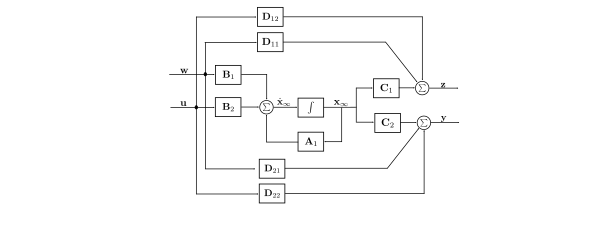
\includegraphics[width=0.6\textwidth]{figures/HinfDiag}
    \end{figure}    
\end{frame}




\definecolor{aaublue}{RGB}{33,26,82}% dark blue

\begin{frame}{Agenda}{}
    \begin{itemize}
        \item Introduction
        \item System Description
        \item Model
        \item Control Approach
        \item Sensor Fusion
        \item \textcolor{aaublue}{\textbf{Inner Controller}}
        \begin{itemize}
            \item[-] Robust Controller Design
            \item[-] \textcolor{aaublue}{\textbf{Linear Quadratic Regulator Design}}
            \item[-] \textcolor{aaublue}{\textbf{Controllers Comparison}}
        \end{itemize}
        \item Outer Controller
        \item Results
        \item Conclusion
    \end{itemize}
\end{frame}
\begin{frame}{Inner Controller}{Linear Quadratic Controller Design}
    
\end{frame}

\begin{frame}{Inner Controller}{Comparison of the Controllers}
    
\end{frame}

\begin{frame}{Agenda}{}
    \begin{itemize}
        \item Introduction
        \item System Description
        \item Model
        \item Control Approach
        \item Sensor Fusion
        \item Inner Controller
        \item \textbf{Outer Controller}
        \begin{itemize}
            \item[-] \textbf{Path Generation Algorithm}
            \item[-] \textbf{Path Following Algorithm}
        \end{itemize}
        \item \textbf{Results}
        \begin{itemize}
            \item[-] \textbf{Simulation Results}
            \item[-] \textbf{Implementation Results}
        \end{itemize}
        \item \textbf{Conclusion}
    \end{itemize}
\end{frame}
%%%%%%%%%%%%%%%%
\section{Outer Controller}

\begin{frame}{Outer Controller}{}

\end{frame}

\begin{frame}{Outer Controller}{Path Generation Algorithm}
    
\end{frame}

\begin{frame}{Outer Controller}{Path Following Algorithm}
    
\end{frame}

%%%%%%%%%%%%%%%%
\section{Results}

\begin{frame}{Results}{Simulation Results}
    
\end{frame}

\begin{frame}{Results}{Implementation Results}
    
\end{frame}

%%%%%%%%%%%%%%%%
\section{Conclusion}

\begin{frame}{Conclusion}{}
    
\end{frame}

%{\aauwavesbg
\begin{frame}[plain,noframenumbering]
    \finalpage{\large{Precision Control of an Autonomous Surface Vessel}}
\end{frame}%}

\end{document}
